\documentclass{article}
\usepackage[utf8]{inputenc}

\title{EE568-HW1-Torque in a Variable Reluctance Machine}
\author{Hakan Polat-2031243 }
\date{07.03.2020}

\usepackage{natbib}
\usepackage{graphicx}

\begin{document}

\maketitle

\section{Introduction}
In this report a variable reluctance machine is investigated both analytically and numerically. In the first part, the system parameters will be delivered. In the next part, an analytic derivation for the reluctance and inductance will be made for the machine under investigation. The torque produced under DC excitation will be derived and presented. Then additional methods for improving the analitic approach will be discussed.\\
In the next part, results for 2D finite element model of the machine will be presented. The analysis is done in ANSYS Maxwell environment. The core material is selected as laminated steel and the permeability is taken as linear. The flux densities for degrees 0,45 and 90 are plotted. The inductance, stored energy and torque is calculated using finite element analysis. The results are then compared to the analytical results and the differences are discussed. \\
In the final part, a non-linear core material is selected. The effect of core saturation is observed. The analysis performed in previous section is repeated. Again the analysis results are compared to the analytical model and the linear core material cases and discussed.

\section{System Parameters and Dimensions}
The variable inductance machine under investigation is presented in Fig. \ref{fig:system}. The machine constist of three parts. The coil windings are used to generated flux. The core is used to direct the flux and torque generated on the rotational section. The coils are wound within 30~mmx10~mm rectangle, each airgap clearance is 0.5~mm, depth of the core is 20~mm, number of turns is 250 and the excitation current is 3A~DC.
\begin{figure}[h!]
	\centering
	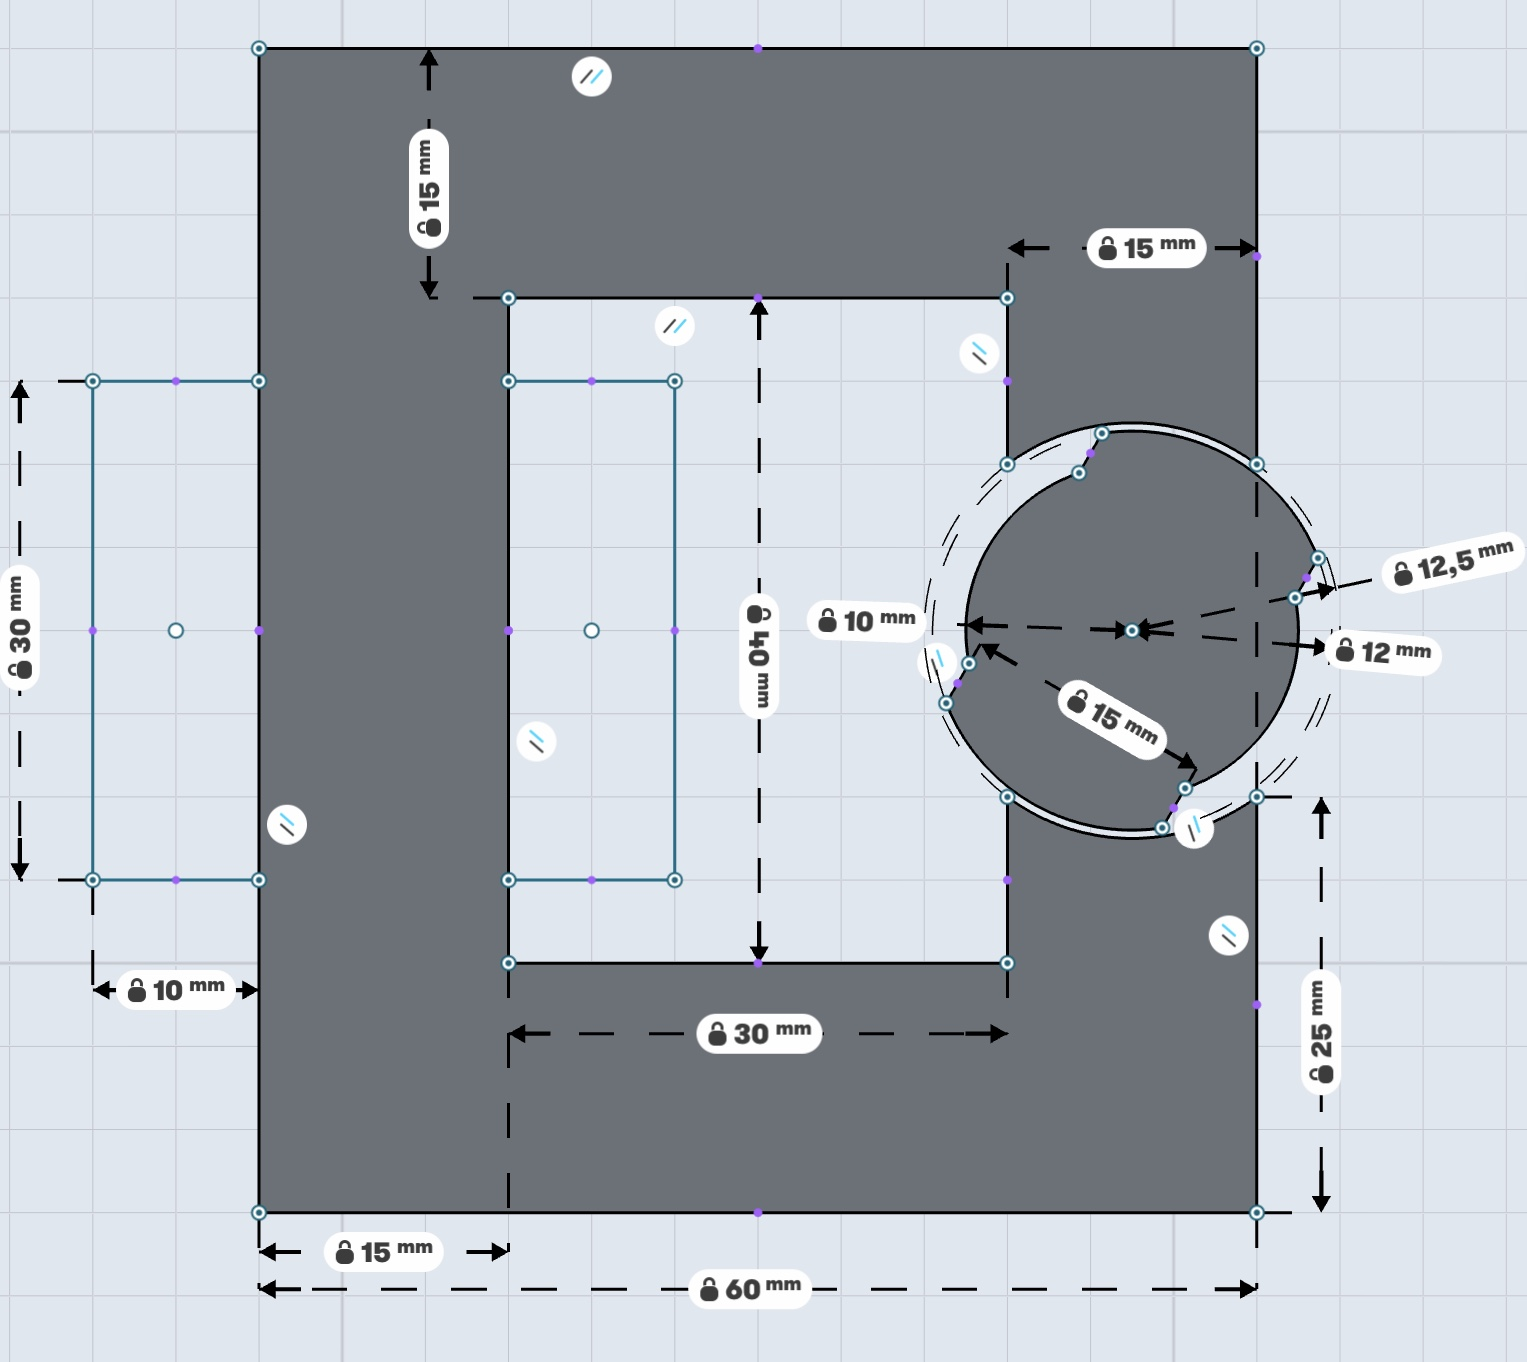
\includegraphics[width=1\linewidth]{Figurler/system.jpeg}
	\caption{2D CAD drawing of the variable reluctance machine under investigation.}
	\label{fig:system}
\end{figure}



\section{Conclusion}

asdadasdas

\end{document}
